\documentclass[]{elsarticle} %review=doublespace preprint=single 5p=2 column
%%% Begin My package additions %%%%%%%%%%%%%%%%%%%
\usepackage[hyphens]{url}
\usepackage{lineno} % add
\providecommand{\tightlist}{%
  \setlength{\itemsep}{0pt}\setlength{\parskip}{0pt}}

\bibliographystyle{elsarticle-harv}
\biboptions{sort&compress} % For natbib
\usepackage{graphicx}
\usepackage{booktabs} % book-quality tables
%% Redefines the elsarticle footer
%\makeatletter
%\def\ps@pprintTitle{%
% \let\@oddhead\@empty
% \let\@evenhead\@empty
% \def\@oddfoot{\it \hfill\today}%
% \let\@evenfoot\@oddfoot}
%\makeatother

% A modified page layout
\textwidth 6.75in
\oddsidemargin -0.15in
\evensidemargin -0.15in
\textheight 9in
\topmargin -0.5in
%%%%%%%%%%%%%%%% end my additions to header

\usepackage[T1]{fontenc}
\usepackage{lmodern}
\usepackage{amssymb,amsmath}
\usepackage{ifxetex,ifluatex}
\usepackage{fixltx2e} % provides \textsubscript
% use upquote if available, for straight quotes in verbatim environments
\IfFileExists{upquote.sty}{\usepackage{upquote}}{}
\ifnum 0\ifxetex 1\fi\ifluatex 1\fi=0 % if pdftex
  \usepackage[utf8]{inputenc}
\else % if luatex or xelatex
  \usepackage{fontspec}
  \ifxetex
    \usepackage{xltxtra,xunicode}
  \fi
  \defaultfontfeatures{Mapping=tex-text,Scale=MatchLowercase}
  \newcommand{\euro}{€}
\fi
% use microtype if available
\IfFileExists{microtype.sty}{\usepackage{microtype}}{}
\usepackage{color}
\usepackage{fancyvrb}
\newcommand{\VerbBar}{|}
\newcommand{\VERB}{\Verb[commandchars=\\\{\}]}
\DefineVerbatimEnvironment{Highlighting}{Verbatim}{commandchars=\\\{\}}
% Add ',fontsize=\small' for more characters per line
\usepackage{framed}
\definecolor{shadecolor}{RGB}{248,248,248}
\newenvironment{Shaded}{\begin{snugshade}}{\end{snugshade}}
\newcommand{\KeywordTok}[1]{\textcolor[rgb]{0.13,0.29,0.53}{\textbf{{#1}}}}
\newcommand{\DataTypeTok}[1]{\textcolor[rgb]{0.13,0.29,0.53}{{#1}}}
\newcommand{\DecValTok}[1]{\textcolor[rgb]{0.00,0.00,0.81}{{#1}}}
\newcommand{\BaseNTok}[1]{\textcolor[rgb]{0.00,0.00,0.81}{{#1}}}
\newcommand{\FloatTok}[1]{\textcolor[rgb]{0.00,0.00,0.81}{{#1}}}
\newcommand{\ConstantTok}[1]{\textcolor[rgb]{0.00,0.00,0.00}{{#1}}}
\newcommand{\CharTok}[1]{\textcolor[rgb]{0.31,0.60,0.02}{{#1}}}
\newcommand{\SpecialCharTok}[1]{\textcolor[rgb]{0.00,0.00,0.00}{{#1}}}
\newcommand{\StringTok}[1]{\textcolor[rgb]{0.31,0.60,0.02}{{#1}}}
\newcommand{\VerbatimStringTok}[1]{\textcolor[rgb]{0.31,0.60,0.02}{{#1}}}
\newcommand{\SpecialStringTok}[1]{\textcolor[rgb]{0.31,0.60,0.02}{{#1}}}
\newcommand{\ImportTok}[1]{{#1}}
\newcommand{\CommentTok}[1]{\textcolor[rgb]{0.56,0.35,0.01}{\textit{{#1}}}}
\newcommand{\DocumentationTok}[1]{\textcolor[rgb]{0.56,0.35,0.01}{\textbf{\textit{{#1}}}}}
\newcommand{\AnnotationTok}[1]{\textcolor[rgb]{0.56,0.35,0.01}{\textbf{\textit{{#1}}}}}
\newcommand{\CommentVarTok}[1]{\textcolor[rgb]{0.56,0.35,0.01}{\textbf{\textit{{#1}}}}}
\newcommand{\OtherTok}[1]{\textcolor[rgb]{0.56,0.35,0.01}{{#1}}}
\newcommand{\FunctionTok}[1]{\textcolor[rgb]{0.00,0.00,0.00}{{#1}}}
\newcommand{\VariableTok}[1]{\textcolor[rgb]{0.00,0.00,0.00}{{#1}}}
\newcommand{\ControlFlowTok}[1]{\textcolor[rgb]{0.13,0.29,0.53}{\textbf{{#1}}}}
\newcommand{\OperatorTok}[1]{\textcolor[rgb]{0.81,0.36,0.00}{\textbf{{#1}}}}
\newcommand{\BuiltInTok}[1]{{#1}}
\newcommand{\ExtensionTok}[1]{{#1}}
\newcommand{\PreprocessorTok}[1]{\textcolor[rgb]{0.56,0.35,0.01}{\textit{{#1}}}}
\newcommand{\AttributeTok}[1]{\textcolor[rgb]{0.77,0.63,0.00}{{#1}}}
\newcommand{\RegionMarkerTok}[1]{{#1}}
\newcommand{\InformationTok}[1]{\textcolor[rgb]{0.56,0.35,0.01}{\textbf{\textit{{#1}}}}}
\newcommand{\WarningTok}[1]{\textcolor[rgb]{0.56,0.35,0.01}{\textbf{\textit{{#1}}}}}
\newcommand{\AlertTok}[1]{\textcolor[rgb]{0.94,0.16,0.16}{{#1}}}
\newcommand{\ErrorTok}[1]{\textcolor[rgb]{0.64,0.00,0.00}{\textbf{{#1}}}}
\newcommand{\NormalTok}[1]{{#1}}
\usepackage{longtable}
\usepackage{graphicx}
% We will generate all images so they have a width \maxwidth. This means
% that they will get their normal width if they fit onto the page, but
% are scaled down if they would overflow the margins.
\makeatletter
\def\maxwidth{\ifdim\Gin@nat@width>\linewidth\linewidth
\else\Gin@nat@width\fi}
\makeatother
\let\Oldincludegraphics\includegraphics
\renewcommand{\includegraphics}[1]{\Oldincludegraphics[width=\maxwidth]{#1}}
\ifxetex
  \usepackage[setpagesize=false, % page size defined by xetex
              unicode=false, % unicode breaks when used with xetex
              xetex]{hyperref}
\else
  \usepackage[unicode=true]{hyperref}
\fi
\hypersetup{breaklinks=true,
            bookmarks=true,
            pdfauthor={},
            pdftitle={Mimicing S\&P 500 Returns via eGARCH and DCC models},
            colorlinks=true,
            urlcolor=blue,
            linkcolor=magenta,
            pdfborder={0 0 0}}
\urlstyle{same}  % don't use monospace font for urls
\setlength{\parindent}{0pt}
\setlength{\parskip}{6pt plus 2pt minus 1pt}
\setlength{\emergencystretch}{3em}  % prevent overfull lines
\setcounter{secnumdepth}{0}
% Pandoc toggle for numbering sections (defaults to be off)
\setcounter{secnumdepth}{0}
% Pandoc header


\usepackage[nomarkers]{endfloat}

\begin{document}
\begin{frontmatter}

  \title{Mimicing S\&P 500 Returns via eGARCH and DCC models}
    \author[]{Nathan Matare}
  
  
      \address[]{The University of Chicago Booth School of Business}
    \address[Another University]{nmatare@chicagobooth.edu}
  
  \begin{abstract}
  Create a portfolio that best mimics the monthly returns of the S\&P 500
  Index over the past 10 years and does not hold more than 10 securities
  at any one time. Securities may consist of individual company stocks and
  not funds or any other type of investment vehicle.
  \end{abstract}
  
 \end{frontmatter}

\section{Methodology}\label{methodology}

In order to appropiately mimic the daily returns of the S\&P 500, one
must isolate secruities whose returns are ``most like'' the S\&P 500 at
any given point in time. By selecting ten secruites who most mirror the
index, one can form a comparable(in returns) profolio.

Whily various metrics such as cointegration and PCA could be considered
as a similarity criterion, I employ dynamic time varying conditional
correlation (DCC) models in order to find and select the most benefical
secruties. This is a non-trivial process; I outline five steps:

\begin{enumerate}
\def\labelenumi{\arabic{enumi}.}
\tightlist
\item
  Collect daily stock level prices on S\&P 500 secruities
\item
  Clean and pre-process data
\item
  Estimate time varying conditional correlation via eGARCH and DCC
  models
\item
  Isolate the top-ten most correlated secruites and form a daily
  profolio
\item
  Compare profolio returns to S\&P 500 returns
\end{enumerate}

First, a targeted universe of secruities is generated. Secondly, the raw
price levels are cleaned, pre-processed, and transformed in order to
faciliate smooth analysis. I next consider several GARCH
models\footnote{GARCH, APARCH, GJG-GARCH, EGARCH are considered} in
order to accurately capture the variance dynamics of each time series;
after compleletion, an appropiate VAR DCC model is fit to the secruity
and market timeseries. Next, the top-ten most correlated secruties are
selected and used as the basis for a daily profolio. Finally, the
profolio returns are compared against daily S\&P 500 returns.

\section{Collect Daily Price Levels}\label{collect-daily-price-levels}

I begin by compiling all stocks currrently listed on the S\&P 500. These
stocks constitute a `universe' of secruities, and form the basis of
candidate secruites. In order to expediate the data collection process,
I write a function ``SecruityScraper''\footnote{See appendix for
  additional information} to scrape daily price level data for the past
10 years.\footnote{See \href{https://www.quandl.com/data/WIKI}{Quandl}
  datasets}

\begin{Shaded}
\begin{Highlighting}[]
\NormalTok{enddate <-}\StringTok{ }\KeywordTok{Sys.Date}\NormalTok{()}
\NormalTok{startdate <-}\StringTok{ }\NormalTok{enddate -}\StringTok{ }\DecValTok{365}\NormalTok{*}\DecValTok{10} 
\KeywordTok{source}\NormalTok{(}\StringTok{"secruityscraper.R"}\NormalTok{)}
\KeywordTok{SecruityScraper}\NormalTok{(}\DataTypeTok{name=}\StringTok{"SP500"}\NormalTok{, }
                \DataTypeTok{startdate=}\NormalTok{startdate, }
                \DataTypeTok{enddate=}\NormalTok{enddate, }\DataTypeTok{type=}\StringTok{"WIKI"}\NormalTok{, }
                \DataTypeTok{key=}\StringTok{"X"}\NormalTok{, }\DataTypeTok{sleep=}\DecValTok{0}\NormalTok{)}
\end{Highlighting}
\end{Shaded}

\section{Collect Daily Price Levels}\label{collect-daily-price-levels-1}

Because the raw data contains weekends, holidays, and missing
observations it is necessary to clean and preprocess the data in order
to faciliate smooth analysis. I write another function,
``SecruityCleaner''\footnote{See appendix for additional information} to
clean the data. \footnote{Missing observations are imputed with either
  the nearest column value or column mean, depedent on the situation,
  see appendix for code logic} Secruites that have too few observations
are removed from the candidate pool; the universe of secruties totals
474.

\begin{Shaded}
\begin{Highlighting}[]
\KeywordTok{source}\NormalTok{(}\StringTok{"secruitycleaner.R"}\NormalTok{)}
\KeywordTok{SecruityCleaner}\NormalTok{(}\DataTypeTok{name=}\StringTok{"SP500"}\NormalTok{, }\DataTypeTok{days=}\DecValTok{144}\NormalTok{)}
\end{Highlighting}
\end{Shaded}

During this step, I append daily S\&P 500 price levels in order to
compare the returns of the formed profolio against the index.

\begin{Shaded}
\begin{Highlighting}[]
\NormalTok{sp <-}\StringTok{ }\KeywordTok{Quandl}\NormalTok{(}\StringTok{"YAHOO/INDEX_GSPC"}\NormalTok{, }\DataTypeTok{start_date=}\NormalTok{startdate, }\DataTypeTok{end_date=}\NormalTok{enddate)}

\NormalTok{rows <-}\StringTok{ }\KeywordTok{match}\NormalTok{(}\KeywordTok{as.character}\NormalTok{(sp[,}\DecValTok{1}\NormalTok{]), }\KeywordTok{as.character}\NormalTok{(raw[,}\DecValTok{1}\NormalTok{])) }\CommentTok{#match SP levels to clean dataset}

\NormalTok{raw$SP500 <-}\StringTok{ }\NormalTok{sp[,}\DecValTok{2}\NormalTok{] }\CommentTok{#append S&P 500 to vector }
\end{Highlighting}
\end{Shaded}

The dataset now contains the entire universe of cleaned secruties and
S\&P 500 price levels. I further manipulate the data by taking the
natural log of the price levels; after differencing the data, I am able
to take advantage of a natural property of logs. I now have a
continously compounded time series.

\[r=ln(p_{t}) - ln(p_{t-1})\]

\begin{Shaded}
\begin{Highlighting}[]
\CommentTok{#Convert data to log level and take difference}
\NormalTok{data <-}\StringTok{ }\KeywordTok{data.frame}\NormalTok{(}\KeywordTok{apply}\NormalTok{(raw[,-}\DecValTok{1}\NormalTok{], }\DataTypeTok{MARGIN=}\DecValTok{2}\NormalTok{, log)) }
\NormalTok{data$Date <-}\StringTok{ }\KeywordTok{as.character}\NormalTok{(dates)}

\CommentTok{#Difference log prices to find returns }
\NormalTok{rtrn <-}\StringTok{ }\KeywordTok{data.frame}\NormalTok{(}\KeywordTok{apply}\NormalTok{(data[,-}\KeywordTok{dim}\NormalTok{(data)[}\DecValTok{2}\NormalTok{]], }\DataTypeTok{MARGIN=}\DecValTok{2}\NormalTok{, diff)) }
\NormalTok{rtrn$Date <-}\StringTok{ }\KeywordTok{as.character}\NormalTok{(dates[-}\DecValTok{1}\NormalTok{])}
\KeywordTok{rownames}\NormalTok{(rtrn) <-}\StringTok{ }\NormalTok{sp$Date[-}\DecValTok{1}\NormalTok{]}
\end{Highlighting}
\end{Shaded}

\section{Analysis: Conditional
Correlations}\label{analysis-conditional-correlations}

This analysis will become computationally expensive. I create a parallel
environment in order to increase the speed of computation.

\begin{Shaded}
\begin{Highlighting}[]
\KeywordTok{library}\NormalTok{(parallel)}
\NormalTok{cl <-}\StringTok{ }\KeywordTok{makeCluster}\NormalTok{(}\KeywordTok{min}\NormalTok{(}\KeywordTok{detectCores}\NormalTok{(),}\DecValTok{5}\NormalTok{),}
      \DataTypeTok{type=}\KeywordTok{ifelse}\NormalTok{(.Platform$OS.type==}\StringTok{"unix"}\NormalTok{,}\StringTok{"FORK"}\NormalTok{,}\StringTok{"PSOCK"}\NormalTok{))}
\end{Highlighting}
\end{Shaded}

In order to fit DCC models to each respective secruity and S\&P 500
index, I first estimate two univariate GARCH models in order to capture
the variance dynamics of each series.

I observe non-normality upon inspection of the raw logged returns. That
is, a fat left-tail. Given this non-normality, it may be that I must
relax normality assumption on my GARCH episolon errors and choose a more
appropiate distribution.

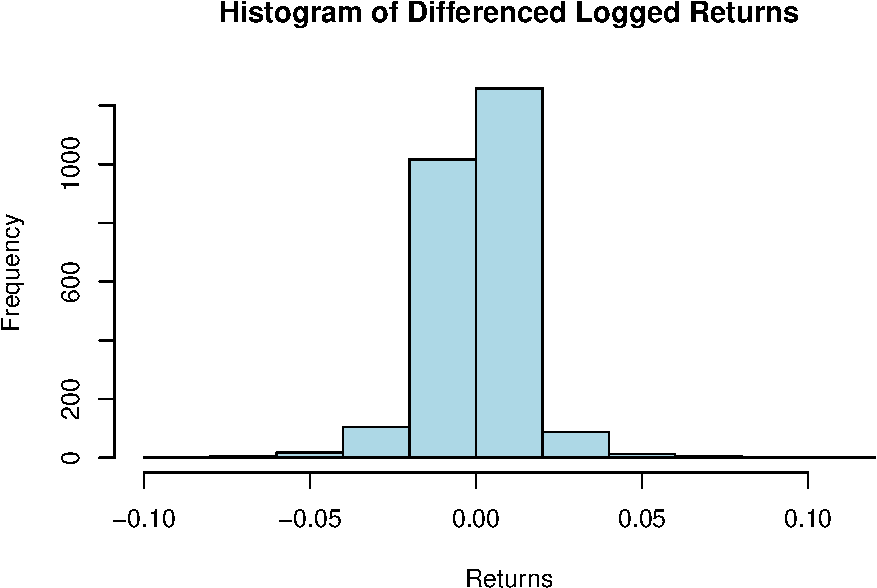
\includegraphics{report_files/figure-latex/analysis11-1.pdf}

\begin{Shaded}
\begin{Highlighting}[]
\KeywordTok{library}\NormalTok{(moments)}
\KeywordTok{kurtosis}\NormalTok{(moddata[,}\DecValTok{1}\NormalTok{])}
\end{Highlighting}
\end{Shaded}

\begin{verbatim}
## [1] 12.93363
\end{verbatim}

\begin{Shaded}
\begin{Highlighting}[]
\KeywordTok{skewness}\NormalTok{(moddata[,}\DecValTok{1}\NormalTok{])}
\end{Highlighting}
\end{Shaded}

\begin{verbatim}
## [1] -0.3189841
\end{verbatim}

I consider asymettric EGARCH, GJG-GARCH, APARCH models and the GARCH
model while varying lagged orders and error distributions: (normal,
normal-skewed, t-distribution, t-skewed) before settling on a
EGARCH(2,2) for the S\&P 500 index and a EGARCH(1,1) for all individual
secruities.

put in latex for EGARCH model

It is unsurprising that an assymetric model works well here; times of
high variance correlation etc\ldots{} talk about what the model is
doing.

Due to computational and time limitations, I blanket an EGARCH(1,1) to
all individual secruites; while most GARCH processes are of either order
(1,1) or (2,2), I have drawn a blanket statement and assummed that all
secruites will follow this process. This is highly uncertain.

In fact, through dianoistic checking I determine that an GRG-GARCH(1,1)
fits mosts series better than any other GARCH process; however when
piping the assymetric process into a DCC model, inverse singular matrix
errors force adoptation of a slightly less complicated model.

\begin{Shaded}
\begin{Highlighting}[]
\KeywordTok{library}\NormalTok{(rmgarch)}
\KeywordTok{require}\NormalTok{(rugarch)}

\CommentTok{#Build parameters for market GARCH}
        \NormalTok{spec1 <-}\StringTok{ }\KeywordTok{ugarchspec}\NormalTok{(}\DataTypeTok{variance.model =} \KeywordTok{list}\NormalTok{(}\DataTypeTok{model =} \StringTok{"eGARCH"}\NormalTok{, }\DataTypeTok{garchOrder =} \KeywordTok{c}\NormalTok{(}\DecValTok{2}\NormalTok{,}\DecValTok{2}\NormalTok{)),}
                                \DataTypeTok{distribution.model=} \StringTok{"norm"}\NormalTok{)}
        
\CommentTok{#Build parameters for secruity GARCH}
        \NormalTok{spec2 <-}\StringTok{ }\KeywordTok{ugarchspec}\NormalTok{(}\DataTypeTok{variance.model =} \KeywordTok{list}\NormalTok{(}\DataTypeTok{model =} \StringTok{"eGARCH"}\NormalTok{, }\DataTypeTok{garchOrder =} \KeywordTok{c}\NormalTok{(}\DecValTok{1}\NormalTok{,}\DecValTok{1}\NormalTok{)),}
                                \DataTypeTok{distribution.model=} \StringTok{"norm"}\NormalTok{)}

\CommentTok{#Fit GARCH models}
        \NormalTok{garch1 <-}\StringTok{ }\KeywordTok{ugarchfit}\NormalTok{(}\DataTypeTok{spec=}\NormalTok{spec1, }\DataTypeTok{data=}\NormalTok{moddata[,}\DecValTok{1}\NormalTok{], }\DataTypeTok{solver.control =} \KeywordTok{list}\NormalTok{(}\DataTypeTok{trace=}\DecValTok{0}\NormalTok{), }
                            \DataTypeTok{cluster=}\NormalTok{cl)}
        \NormalTok{garch2 <-}\StringTok{ }\KeywordTok{try}\NormalTok{(}\KeywordTok{ugarchfit}\NormalTok{(}\DataTypeTok{spec=}\NormalTok{spec2, }\DataTypeTok{data=}\NormalTok{moddata[,}\DecValTok{2}\NormalTok{], }\DataTypeTok{solver.control =} \KeywordTok{list}\NormalTok{(}\DataTypeTok{trace=}\DecValTok{0}\NormalTok{), }
                            \DataTypeTok{cluster=}\NormalTok{cl), }\DataTypeTok{silent=}\OtherTok{TRUE}\NormalTok{)}
\end{Highlighting}
\end{Shaded}

Before continuing, I conduct several quick diagnostic checks. My S\&P
500 EGARCH(2,2) process captures all serial correlation in the time
series. While I cannot confirm that each individaul secruity follows a
EGARCH(1,1) process, I accept this assumption given time and
computational constrains and proceed with the analysis.

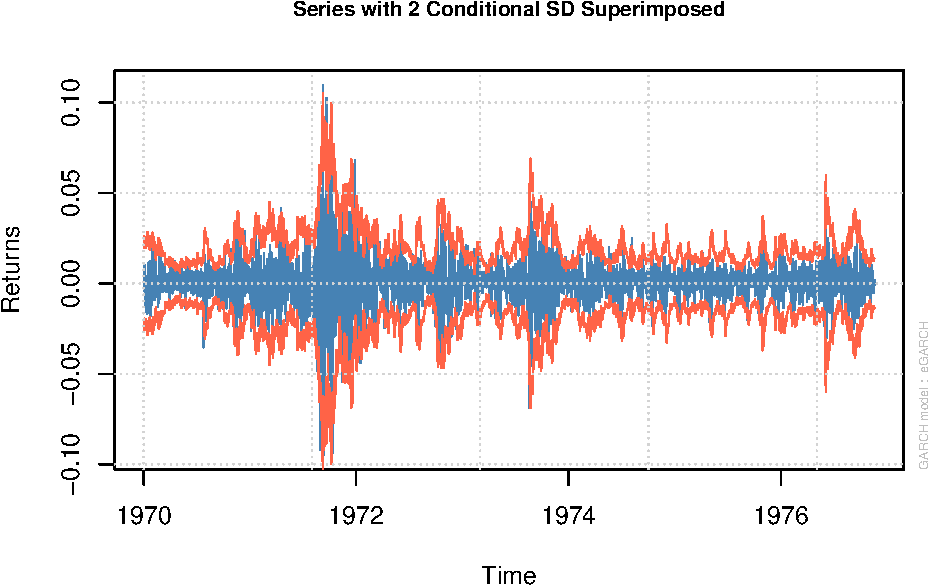
\includegraphics{report_files/figure-latex/analysis201-1.pdf}

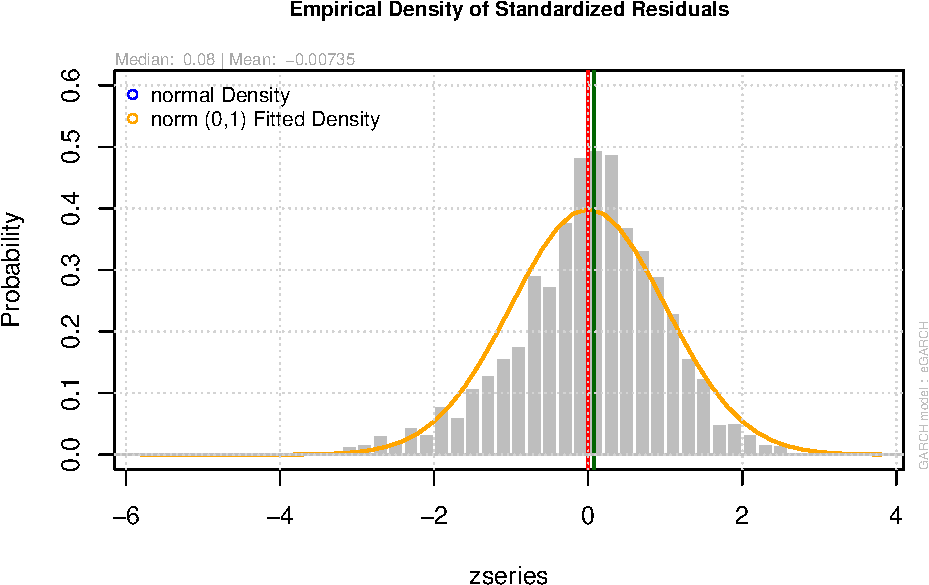
\includegraphics{report_files/figure-latex/analysis20df1-1.pdf}

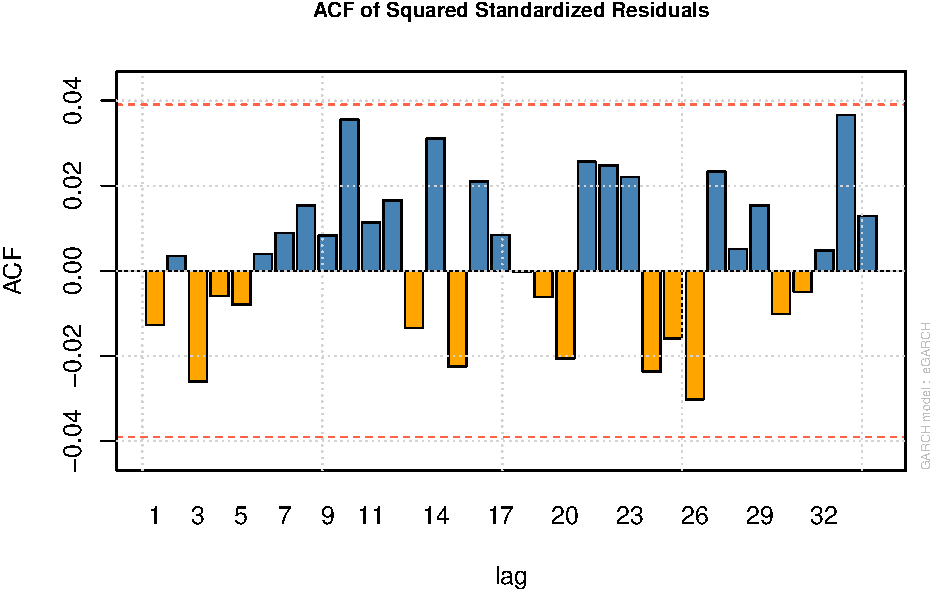
\includegraphics{report_files/figure-latex/analysis2031-1.pdf}

Although heavy left skew remains in my residuals--indicative of a
less-than-perfect fit ARCH model, these are the best results I am able
to get.

While the residual errors are not perfectly normally distributed,
relaxing the assumption and estimating student-t or skewed-normal
distrubtion worsens the kurtosis and skewness. I proceed under the
normal assumption.

\begin{Shaded}
\begin{Highlighting}[]
\KeywordTok{kurtosis}\NormalTok{(garch1@fit$residuals)}
\end{Highlighting}
\end{Shaded}

\begin{verbatim}
## [1] 12.63651
\end{verbatim}

\begin{Shaded}
\begin{Highlighting}[]
\KeywordTok{skewness}\NormalTok{(garch1@fit$residuals)}
\end{Highlighting}
\end{Shaded}

\begin{verbatim}
## [1] -0.4385969
\end{verbatim}

Inspecting the EGARCH(2,2) S\&P 500 coefficients, I observe significant
covariates. Notably the assymetric terms(gamma, and gamma2) are highly
signifcant.

Inspecting, the EGARCH(1,1) individaul secruity coefficients, I observe
highly significant covariates with the expection of the long-run mean
(mu). It would appear to indicate that there is no long-run
mean-variance for this secruity--at least one estimated by statistically
sound parameters.

\begin{longtable}[c]{@{}lrrrr@{}}
\toprule
& Estimate & Std. Error & t value &
Pr(\textgreater{}\textbar{}t\textbar{})\tabularnewline
\midrule
\endhead
mu & 0.0002682 & 0.0001182 & 2.269900 & 0.0232137\tabularnewline
ar1 & 0.3271671 & 0.0554327 & 5.902059 & 0.0000000\tabularnewline
ma1 & -0.3909436 & 0.0537169 & -7.277854 & 0.0000000\tabularnewline
omega & -0.2859863 & 0.0179554 & -15.927569 & 0.0000000\tabularnewline
alpha1 & -0.2968012 & 0.0303461 & -9.780529 & 0.0000000\tabularnewline
alpha2 & 0.1269753 & 0.0272309 & 4.662917 & 0.0000031\tabularnewline
beta1 & 0.9999999 & 0.0000088 & 113420.181733 & 0.0000000\tabularnewline
beta2 & -0.0312999 & 0.0019570 & -15.993674 & 0.0000000\tabularnewline
gamma1 & -0.1449825 & 0.0391676 & -3.701592 & 0.0002143\tabularnewline
gamma2 & 0.2973042 & 0.0425145 & 6.993006 & 0.0000000\tabularnewline
\bottomrule
\end{longtable}

\begin{longtable}[c]{@{}lrrrr@{}}
\toprule
& Estimate & Std. Error & t value &
Pr(\textgreater{}\textbar{}t\textbar{})\tabularnewline
\midrule
\endhead
mu & 0.0000000 & 0.0000006 & 0.0000047 & 0.9999962\tabularnewline
ar1 & 0.3685570 & 0.0319029 & 11.5524440 & 0.0000000\tabularnewline
ma1 & -0.6756093 & 0.0083962 & -80.4663500 & 0.0000000\tabularnewline
omega & -0.4826973 & 0.0193245 & -24.9785618 & 0.0000000\tabularnewline
alpha1 & 0.1133147 & 0.0264116 & 4.2903325 & 0.0000178\tabularnewline
beta1 & 0.9002138 & 0.0012210 & 737.2798943 & 0.0000000\tabularnewline
gamma1 & 1.4878254 & 0.0442731 & 33.6056502 & 0.0000000\tabularnewline
\bottomrule
\end{longtable}

Now that i have finished estimating univariate variances, I am ready to
incorporate this information into a multivariate DCC model. Although I
had considered asymmetric variance dynamics in the previous EGARCH
estimations, I discard an aDCC model due to its insignificant
coefficients and non-intuitive understanding.

``Include Equation description here''"

Diagnostic checking here indicates that a mulitvariate DCC(1,1) model is
the most suitable for this process, while higher orders models appear to
have comproable BIC/AIC scores, and better fit to the skewed, non-normal
data-- the higher order coefficients are insignicant and I fear that I
risk overfitting at this point.

After fitting the model, I construct the correlation matrix and
terminate the parralel cluster.

\begin{Shaded}
\begin{Highlighting}[]
\CommentTok{#Build parameters for DCC model }
\NormalTok{dccspec <-}\StringTok{ }\KeywordTok{dccspec}\NormalTok{(}\DataTypeTok{VAR=}\OtherTok{TRUE}\NormalTok{, }\DataTypeTok{uspec =} \KeywordTok{multispec}\NormalTok{(}\KeywordTok{c}\NormalTok{(spec1, spec2)), }\DataTypeTok{dccOrder =} \KeywordTok{c}\NormalTok{(}\DecValTok{1}\NormalTok{,}\DecValTok{1}\NormalTok{), }
                   \DataTypeTok{distribution =} \StringTok{"mvnorm"}\NormalTok{)}

\CommentTok{#Fit DCC model}
\NormalTok{dcc <-}\StringTok{ }\KeywordTok{try}\NormalTok{(}\KeywordTok{dccfit}\NormalTok{(dccspec, }\DataTypeTok{data =} \NormalTok{moddata, }\DataTypeTok{fit.control=}\KeywordTok{list}\NormalTok{(}\DataTypeTok{scale=}\OtherTok{TRUE}\NormalTok{), }\DataTypeTok{cluster=}\NormalTok{cl), }
           \DataTypeTok{silent=}\OtherTok{TRUE}\NormalTok{)}

\NormalTok{corrmatrix <-}\StringTok{ }\KeywordTok{rcor}\NormalTok{(dcc, }\DataTypeTok{type=}\StringTok{"R"}\NormalTok{)}
\NormalTok{corrmatrix <-}\StringTok{ }\KeywordTok{zoo}\NormalTok{(corrmatrix[}\DecValTok{1}\NormalTok{,}\DecValTok{2}\NormalTok{,], }\DataTypeTok{order.by=}\KeywordTok{as.Date}\NormalTok{(}\KeywordTok{rownames}\NormalTok{(moddata)))}
\NormalTok{timevarcor[,n] <-}\StringTok{ }\NormalTok{corrmatrix}

\KeywordTok{stopCluster}\NormalTok{(cl) }
\end{Highlighting}
\end{Shaded}

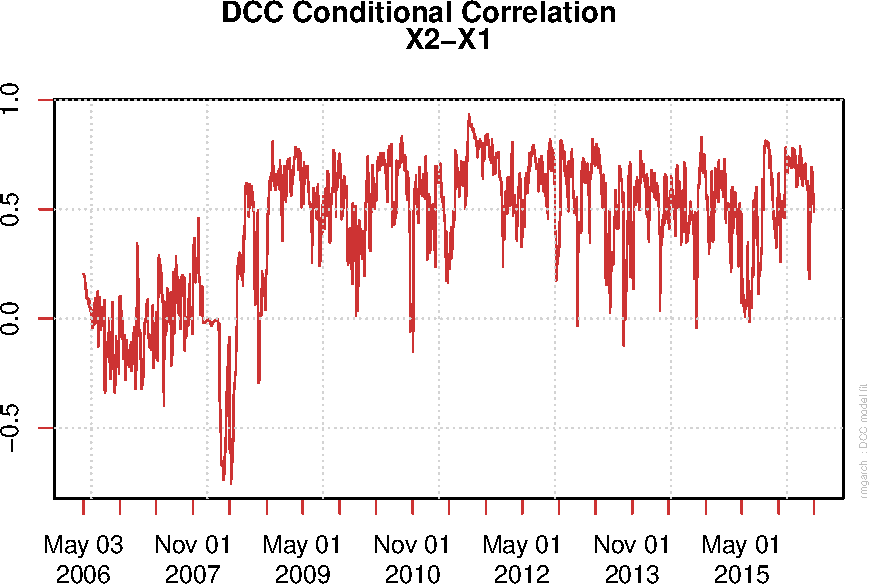
\includegraphics{report_files/figure-latex/analysis232011-1.pdf}

A mulivariate DCC(1,1) indicates that most coefficients are significant,
although I believe I have spurious estimations for the X1/X2 Beta1
coefficient. Individaul secruity coefficients appear to be weaker (X2
variables) than the coefficients fit for the S\&P 500.

\begin{longtable}[c]{@{}lrrrr@{}}
\toprule
& Estimate & Std. Error & t value &
Pr(\textgreater{}\textbar{}t\textbar{})\tabularnewline
\midrule
\endhead
{[}X1{]}.omega & -0.2812474 & 0.0478390 & -5.8790349 &
0.0000000\tabularnewline
{[}X1{]}.alpha1 & -0.2931646 & 0.0282848 & -10.3647370 &
0.0000000\tabularnewline
{[}X1{]}.alpha2 & 0.1245218 & 0.0278806 & 4.4662556 &
0.0000080\tabularnewline
{[}X1{]}.beta1 & 1.0000000 & 0.0000232 & 43143.5149533 &
0.0000000\tabularnewline
{[}X1{]}.beta2 & -0.0309803 & 0.0052412 & -5.9109612 &
0.0000000\tabularnewline
{[}X1{]}.gamma1 & -0.1388295 & 0.0202280 & -6.8632455 &
0.0000000\tabularnewline
{[}X1{]}.gamma2 & 0.2874979 & 0.0294032 & 9.7777600 &
0.0000000\tabularnewline
{[}X2{]}.omega & -0.0115805 & 0.0208363 & -0.5557843 &
0.5783584\tabularnewline
{[}X2{]}.alpha1 & -0.0448929 & 0.1792462 & -0.2504539 &
0.8022364\tabularnewline
{[}X2{]}.beta1 & 0.9977422 & 0.0016093 & 620.0005213 &
0.0000000\tabularnewline
{[}X2{]}.gamma1 & 0.1383119 & 0.1087630 & 1.2716814 &
0.2034863\tabularnewline
{[}Joint{]}dcca1 & 0.1147132 & 0.0295329 & 3.8842557 &
0.0001026\tabularnewline
{[}Joint{]}dccb1 & 0.8813116 & 0.0311983 & 28.2486921 &
0.0000000\tabularnewline
\bottomrule
\end{longtable}

Talka bouthuge matrix of correlationsh now and speak about finding top
10 biggest

\begin{Shaded}
\begin{Highlighting}[]
\NormalTok{top10names <-}\StringTok{ }\KeywordTok{apply}\NormalTok{(timevarcor[,-}\DecValTok{1}\NormalTok{], }\DataTypeTok{MARGIN=}\DecValTok{1}\NormalTok{, }\DataTypeTok{FUN=}\NormalTok{function(x) }
                   \KeywordTok{names}\NormalTok{(}\KeywordTok{head}\NormalTok{(}\KeywordTok{sort}\NormalTok{(x, }\DataTypeTok{decreasing =} \DataTypeTok{decreasing=}\OtherTok{TRUE}\NormalTok{),}\DecValTok{10}\NormalTok{)))}

\CommentTok{#Compare returns against SP&500 Returns}
\NormalTok{L <-}\StringTok{ }\KeywordTok{dim}\NormalTok{(top10names)[}\DecValTok{2}\NormalTok{]}
\NormalTok{eval <-}\StringTok{ }\KeywordTok{data.frame}\NormalTok{(}\DataTypeTok{Date=}\NormalTok{sp$Date[-}\DecValTok{1}\NormalTok{])}
\NormalTok{eval$SP500 <-}\StringTok{ }\NormalTok{rtrn[,}\DecValTok{474}\NormalTok{]}
\NormalTok{eval$benchmark <-}\StringTok{ }\OtherTok{NA}

\NormalTok{for(n in }\DecValTok{1}\NormalTok{:L)\{}
    \NormalTok{date <-}\StringTok{ }\KeywordTok{names}\NormalTok{(top10names[}\DecValTok{1}\NormalTok{,n])}
    \NormalTok{topstocks <-}\StringTok{ }\KeywordTok{as.character}\NormalTok{(top10names[,n])}
    \NormalTok{lowstocks <-}\StringTok{ }\KeywordTok{as.character}\NormalTok{(low10names[,n])}

    \NormalTok{eval$benchmark[n] <-}\StringTok{ }\KeywordTok{mean}\NormalTok{(}\KeywordTok{as.numeric}\NormalTok{(rtrn[date,topstocks]))}
\NormalTok{\}}
\NormalTok{eval$error <-}\StringTok{ }\NormalTok{eval$SP500 -}\StringTok{ }\NormalTok{eval$benchmark }
\end{Highlighting}
\end{Shaded}

Talk about errors and include big graph

\begin{verbatim}
## Warning: Removed 2 rows containing missing values (geom_path).

## Warning: Removed 2 rows containing missing values (geom_path).
\end{verbatim}

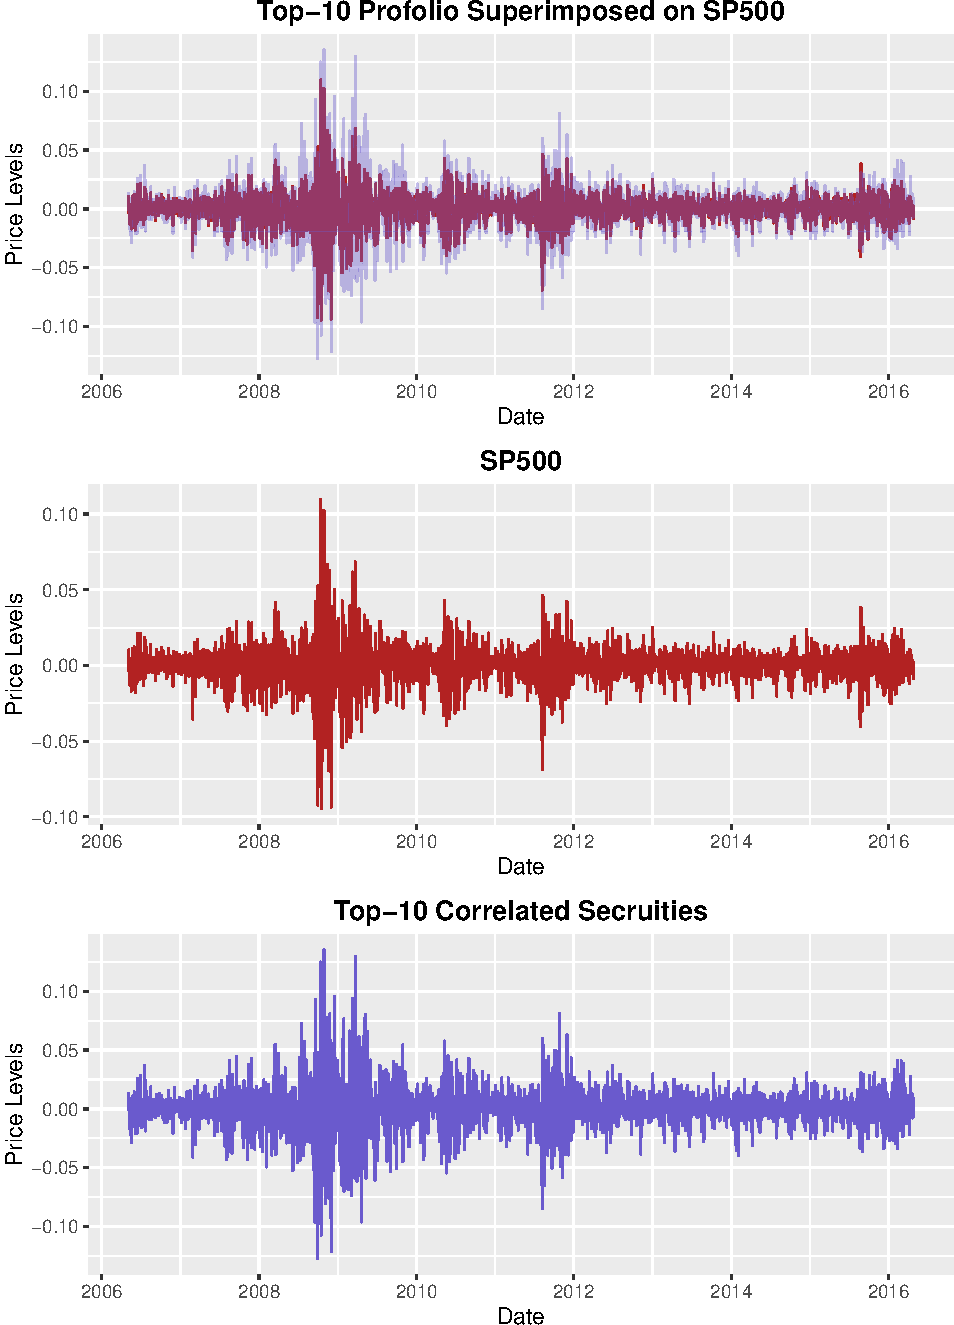
\includegraphics{report_files/figure-latex/analysis23223d011-1.pdf}

talk about getting the top 10 correlations per day

\section{Conclusion}\label{conclusion}

Talk about naive weighting, introduce variable weighting, better model
estimatoin, automatiion of GARCH selection (1,1) assumption, higher
order DCC model?

\section{Appendix}\label{appendix}

\begin{Shaded}
\begin{Highlighting}[]
\NormalTok{SecruityScraper <-}\StringTok{ }\NormalTok{function(name, startdate, enddate, type, key, sleep)\{}

\CommentTok{# Description}
\CommentTok{# This script scraps Quandl.com for data given a date range and symbol list}

\CommentTok{# Arguments}

\CommentTok{#'name' is the name of a csv file containing stock symbols to download #do not include .csv}
\CommentTok{#'startdate' is the start date of data}
\CommentTok{#'enddate' is the end data of data}
\CommentTok{#'type' is the Quandl database header; this should be input as a character  IE 'WIKI'}
\CommentTok{#'key' is the Quandl key}
\CommentTok{#'sleep' is the number of seconds to wait before querying Quandl server}

\CommentTok{# Example}
\CommentTok{# SecruityScraper("NASDAQ", "2001-09-11", "2015-01-01", "WIKI","40F..U&E")}

\CommentTok{# Requirements}

\CommentTok{# Requires the Quandl library}
\CommentTok{# Requires loaded csv file to have a column header of "ticker" for all secruity symbols}
\CommentTok{# Startdate and enddate must not be same date}
                    
\CommentTok{#setup environment}
\NormalTok{name <-}\StringTok{ }\NormalTok{name}
\NormalTok{raw <-}\StringTok{ }\KeywordTok{read.csv}\NormalTok{(}\KeywordTok{paste}\NormalTok{(name,}\StringTok{".csv"}\NormalTok{, }\DataTypeTok{sep=}\StringTok{''}\NormalTok{))}
\NormalTok{tickers <-}\StringTok{ }\KeywordTok{as.character}\NormalTok{(raw$ticker)}

\NormalTok{enddate <-}\StringTok{ }\NormalTok{enddate}
\NormalTok{startdate <-}\StringTok{ }\NormalTok{startdate}
\NormalTok{dates <-}\StringTok{ }\KeywordTok{seq.Date}\NormalTok{(}\KeywordTok{as.Date}\NormalTok{(startdate), }\KeywordTok{as.Date}\NormalTok{(enddate), }\DataTypeTok{by=}\StringTok{'day'}\NormalTok{) }\CommentTok{#create daily dates}

\CommentTok{#allocate memory for data}
\NormalTok{L <-}\StringTok{ }\KeywordTok{length}\NormalTok{(tickers)}
\NormalTok{D <-}\StringTok{ }\KeywordTok{length}\NormalTok{(dates) }
\NormalTok{dataset <-}\StringTok{ }\KeywordTok{matrix}\NormalTok{(}\DataTypeTok{ncol=}\NormalTok{L, }\DataTypeTok{nrow=}\NormalTok{D)}
\KeywordTok{dimnames}\NormalTok{(dataset) <-}\StringTok{ }\KeywordTok{list}\NormalTok{(}\KeywordTok{rownames}\NormalTok{(dataset, }
                                   \DataTypeTok{do.NULL =} \OtherTok{FALSE}\NormalTok{, }
                                   \DataTypeTok{prefix =} \StringTok{"row"}\NormalTok{), }
                                   \KeywordTok{colnames}\NormalTok{(dataset, }
                                   \DataTypeTok{do.NULL =} \OtherTok{FALSE}\NormalTok{, }
                                   \DataTypeTok{prefix =} \StringTok{"col"}\NormalTok{))}
\KeywordTok{colnames}\NormalTok{(dataset) <-}\StringTok{ }\NormalTok{tickers}
\KeywordTok{rownames}\NormalTok{(dataset) <-}\StringTok{ }\KeywordTok{as.character}\NormalTok{(dates)}

\CommentTok{#specify date range}
\NormalTok{enddate <-}\StringTok{ }\NormalTok{dates[}\KeywordTok{length}\NormalTok{(dates)]}
\NormalTok{startdate <-}\StringTok{ }\NormalTok{dates[}\DecValTok{1}\NormalTok{]}
\NormalTok{header <-}\StringTok{ }\KeywordTok{paste}\NormalTok{(type, }\StringTok{"/"}\NormalTok{, }\DataTypeTok{sep=}\StringTok{""}\NormalTok{)}

\CommentTok{#retrive stock data}
\KeywordTok{require}\NormalTok{(Quandl)}
\KeywordTok{Quandl.api_key}\NormalTok{(key)}

\NormalTok{for(i in }\DecValTok{1}\NormalTok{:L)\{}

\KeywordTok{tryCatch}\NormalTok{(\{}
\NormalTok{sym <-}\StringTok{ }\KeywordTok{paste}\NormalTok{(header, tickers[i], }\DataTypeTok{sep=}\StringTok{""}\NormalTok{)}
\NormalTok{info <-}\StringTok{ }\KeywordTok{Quandl}\NormalTok{(sym, }\DataTypeTok{start_date=}\NormalTok{startdate, }\DataTypeTok{end_date=}\NormalTok{enddate)}
\NormalTok{tempdate <-}\StringTok{ }\NormalTok{info$Date}

\NormalTok{info <-}\StringTok{ }\KeywordTok{data.frame}\NormalTok{(info$Close)}
\KeywordTok{rownames}\NormalTok{(info) <-}\StringTok{ }\NormalTok{tempdate}
\NormalTok{put <-}\StringTok{ }\KeywordTok{merge}\NormalTok{(info, dataset[,i], }\DataTypeTok{by=}\DecValTok{0}\NormalTok{, }\DataTypeTok{all=}\OtherTok{TRUE}\NormalTok{)}
\NormalTok{dataset[,i] <-}\StringTok{ }\NormalTok{put$info.Close}
\KeywordTok{message}\NormalTok{(}\StringTok{"Scraping data for stock: "}\NormalTok{, tickers[i], }\StringTok{" | Number: "}\NormalTok{, i, }\StringTok{"/"}\NormalTok{, L)}

\KeywordTok{Sys.sleep}\NormalTok{(sleep) }\CommentTok{#API speed limit }
\NormalTok{\}, }\DataTypeTok{error=}\NormalTok{function(e)    \{}
\KeywordTok{cat}\NormalTok{(}\StringTok{"ERROR :"}\NormalTok{,}\KeywordTok{conditionMessage}\NormalTok{(e), }\StringTok{"}\CharTok{\textbackslash{}n}\StringTok{"}\NormalTok{)}
\CommentTok{#Last value throws error}
\NormalTok{\})}

\NormalTok{\}}

\CommentTok{#export data }
\KeywordTok{write.csv}\NormalTok{(dataset, }\DataTypeTok{file =} \KeywordTok{paste}\NormalTok{(name,}\StringTok{"-output.csv"}\NormalTok{, }\DataTypeTok{sep=}\StringTok{''}\NormalTok{))}

\NormalTok{\}}


\CommentTok{# Utility script for Secruity Cleaner }
\NormalTok{remove_outliers <-}\StringTok{ }\NormalTok{function(x, }\DataTypeTok{na.rm =} \OtherTok{TRUE}\NormalTok{, ...) \{}
  \NormalTok{qnt <-}\StringTok{ }\KeywordTok{quantile}\NormalTok{(x, }\DataTypeTok{probs=}\KeywordTok{c}\NormalTok{(.}\DecValTok{25}\NormalTok{, .}\DecValTok{75}\NormalTok{), }\DataTypeTok{na.rm =} \NormalTok{na.rm, ...)}
  \NormalTok{H <-}\StringTok{ }\FloatTok{1.5} \NormalTok{*}\StringTok{ }\KeywordTok{IQR}\NormalTok{(x, }\DataTypeTok{na.rm =} \NormalTok{na.rm)}
  \NormalTok{y <-}\StringTok{ }\NormalTok{x}
  \NormalTok{y[x <}\StringTok{ }\NormalTok{(qnt[}\DecValTok{1}\NormalTok{] -}\StringTok{ }\NormalTok{H)] <-}\StringTok{ }\OtherTok{NA}
  \NormalTok{y[x >}\StringTok{ }\NormalTok{(qnt[}\DecValTok{2}\NormalTok{] +}\StringTok{ }\NormalTok{H)] <-}\StringTok{ }\OtherTok{NA}
  \NormalTok{y}
\NormalTok{\}}
\end{Highlighting}
\end{Shaded}

\begin{Shaded}
\begin{Highlighting}[]
\NormalTok{SecruityCleaner <-}\StringTok{ }\NormalTok{function(name, days)\{}

\CommentTok{# Description}
\CommentTok{# This utility script removes non-trading days from SecruityScraper and imputes missing values with the nearest value }

\CommentTok{# Arguments}
\CommentTok{#'name' is the name of a csv file containing stock symbols to download #do not include .csv}
\CommentTok{#'days' is the number of expected non-trading days per average year, default is 144}

\CommentTok{# Example}
\CommentTok{# SecruityCleaner("NASDAQ", 144)}

\CommentTok{# Requirements}

\CommentTok{# Requires the zoo library}

\CommentTok{# Other}

\CommentTok{# Error "ERROR(expected) : undefined columns selected" is excpected as columns are removed and length of for-loop does not dynamically change}

\CommentTok{#setup environment}
\NormalTok{raw <-}\StringTok{ }\KeywordTok{read.csv}\NormalTok{(}\KeywordTok{paste}\NormalTok{(name,}\StringTok{"-output.csv"}\NormalTok{, }\DataTypeTok{sep=}\StringTok{''}\NormalTok{))}
\KeywordTok{colnames}\NormalTok{(raw)[}\KeywordTok{colnames}\NormalTok{(raw)==}\StringTok{"X"}\NormalTok{] <-}\StringTok{ "date"}
\NormalTok{L <-}\StringTok{ }\KeywordTok{length}\NormalTok{(raw)}

\CommentTok{# take out the non trading days aka weekends and holidays}
\NormalTok{narows <-}\StringTok{ }\KeywordTok{as.numeric}\NormalTok{(}\KeywordTok{rownames}\NormalTok{(raw[}\KeywordTok{rowSums}\NormalTok{(}\KeywordTok{is.na}\NormalTok{(raw))>=}\KeywordTok{dim}\NormalTok{(raw)[}\DecValTok{2}\NormalTok{]-}\DecValTok{10}\NormalTok{,])) }
\NormalTok{raw <-}\StringTok{ }\NormalTok{raw[-narows,]}
\NormalTok{U <-}\StringTok{ }\KeywordTok{dim}\NormalTok{(raw)[}\DecValTok{1}\NormalTok{]/}\DecValTok{365}\NormalTok{*(days}\DecValTok{-3}\NormalTok{) }\CommentTok{#number of years worth of data * number of non-trading days = max expected NAs #where 3 is a buffer}
\NormalTok{L <-}\StringTok{ }\KeywordTok{length}\NormalTok{(raw)}

\CommentTok{#Remove secruites with missing observations}
\NormalTok{for(n in }\DecValTok{2}\NormalTok{:(L}\DecValTok{-1}\NormalTok{))\{}

  \KeywordTok{tryCatch}\NormalTok{(\{}
        \NormalTok{if (}\KeywordTok{sum}\NormalTok{(}\KeywordTok{is.na}\NormalTok{(raw[,n])) <}\StringTok{ }\NormalTok{U) \{}
                        \KeywordTok{message}\NormalTok{(}\StringTok{"Pass: "}\NormalTok{, n)}
        \NormalTok{\} else \{}
                      \KeywordTok{message}\NormalTok{(}\StringTok{"Remove (not enough observations): "}\NormalTok{, n)}
                        \NormalTok{raw <-}\StringTok{ }\NormalTok{raw[,-}\KeywordTok{c}\NormalTok{(n)]}
        \NormalTok{\}}
    \NormalTok{\}, }\DataTypeTok{error=}\NormalTok{function(e)    \{}\CommentTok{#as columns are strunk, n becomes larger than initial column number set and produces errors at the end}
    \KeywordTok{cat}\NormalTok{(}\StringTok{"ERROR(expected) :"}\NormalTok{,}\KeywordTok{conditionMessage}\NormalTok{(e), }\StringTok{"}\CharTok{\textbackslash{}n}\StringTok{"}\NormalTok{)}
    \NormalTok{\})}

\NormalTok{\}}

\KeywordTok{require}\NormalTok{(zoo)}
\NormalTok{L <-}\StringTok{ }\KeywordTok{length}\NormalTok{(raw)}
\NormalTok{end <-}\StringTok{ }\KeywordTok{dim}\NormalTok{(raw)[}\DecValTok{1}\NormalTok{]}

\CommentTok{#Impute missing price levels with nearest price level}
\NormalTok{for(n in }\DecValTok{2}\NormalTok{:L)\{}

\NormalTok{raw[}\DecValTok{1}\NormalTok{,n] <-}\StringTok{ }\KeywordTok{ifelse}\NormalTok{(}\KeywordTok{is.na}\NormalTok{(raw[}\DecValTok{1}\NormalTok{,n])==}\OtherTok{TRUE}\NormalTok{, }\KeywordTok{na.locf}\NormalTok{(raw[,n])[}\DecValTok{1}\NormalTok{], raw[}\DecValTok{1}\NormalTok{,n]) }\CommentTok{#place value in first }
\NormalTok{raw[end,n] <-}\StringTok{ }\KeywordTok{ifelse}\NormalTok{(}\KeywordTok{is.na}\NormalTok{(raw[end,n])==}\OtherTok{TRUE}\NormalTok{, }\KeywordTok{na.locf}\NormalTok{(raw[,n])[end], raw[end,n]) }\CommentTok{#place value in last}
\NormalTok{raw[,n] <-}\StringTok{ }\KeywordTok{na.locf}\NormalTok{(raw[,n] ,}\DataTypeTok{fromlast=}\OtherTok{TRUE}\NormalTok{) }\CommentTok{# scrub NA from backwards}
\KeywordTok{message}\NormalTok{(}\StringTok{"Imputing missing values with nearest value: "}\NormalTok{, n)}

\NormalTok{\}}

\CommentTok{#Remove outliers and replace them with mean}
\NormalTok{L <-}\StringTok{ }\KeywordTok{length}\NormalTok{(raw)}
\NormalTok{for(n in }\DecValTok{2}\NormalTok{:L)\{}
            \NormalTok{removed <-}\StringTok{ }\KeywordTok{remove_outliers}\NormalTok{(raw[,n])}
            \NormalTok{removed[}\KeywordTok{is.na}\NormalTok{(removed)] =}\StringTok{ }\KeywordTok{mean}\NormalTok{(removed, }\DataTypeTok{na.rm=}\OtherTok{TRUE}\NormalTok{)}
            \NormalTok{raw[,n] <-}\StringTok{ }\NormalTok{removed}
            \KeywordTok{message}\NormalTok{(}\StringTok{"Removing outliers and imputing with mean: "}\NormalTok{, n)}
            \NormalTok{\}}

\KeywordTok{write.csv}\NormalTok{(raw, }\DataTypeTok{file =} \KeywordTok{paste}\NormalTok{(name,}\StringTok{"-output-clean.csv"}\NormalTok{, }\DataTypeTok{sep=}\StringTok{''}\NormalTok{))}

\NormalTok{\}}
\end{Highlighting}
\end{Shaded}

\end{document}


